\subsection{Lukket kabinet}
I denne konfiguration blev alle basrefleks-huller forseglet med propper således, at kabinettet var så godt som lufttæt. Frekvenskarakteristikken blev herefter målt ved, at placere CLIO-mikrofonen lige foran membranen og i 1 meters afstand foran membranen. Resultatet af dette ses på figuren nedenfor.
\begin{figure}[H]
	\centering
	\vspace{-12pt}
	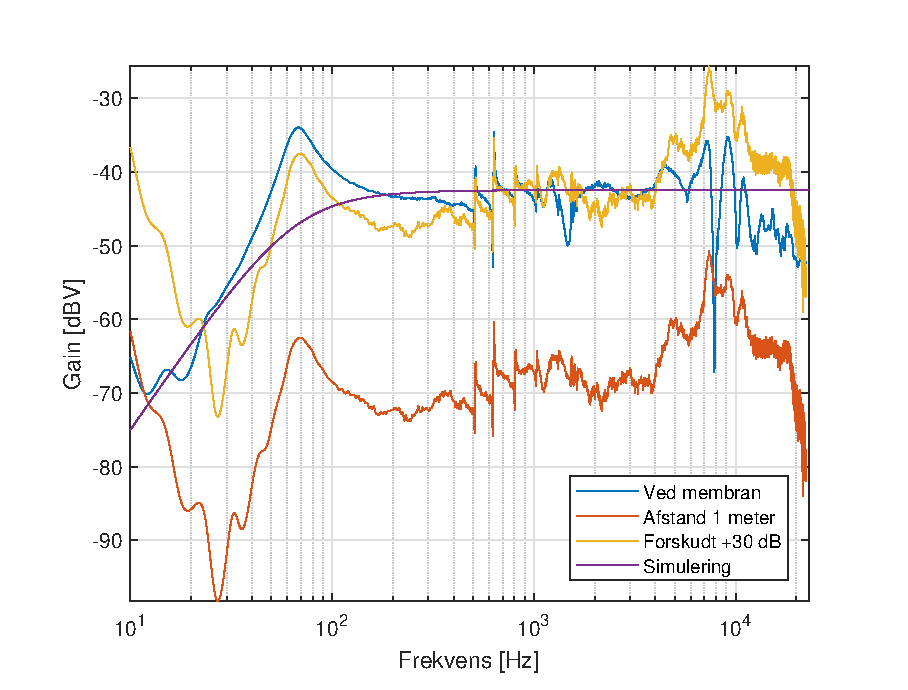
\includegraphics[width=\textwidth]{Pics/ClosedCabinet}
	\caption{Målinger på et lukket kabinet}
\end{figure}

Det ses på figuren at, den første resonansfrekvens $f_s$ ligger ved omkring \SI{70}{\hertz} og at forstærkningen stiger med omkring 18 dB/oktav i det fjederstyrede område - altså området under resonansfrekvensen.

Hvis det antages, at det massestyrede område er omtrent en dekade bred i frekvensspektret, så vil dette område derfor ligge mellem \SI{70}{\hertz} og \SI{700}{\hertz}. Herefter vil direktiviteten begynde at spille en rolle for karakteristikkens udseende.
 
Det ses også, at når CLIO-mikrofonen flyttes længere væk fra membranen, så bevarer karakteristikken nogenlunde sin form i det massestyrede område og et godt stykke ind i både området over og under i frekvensspektret. Den største forskel er dog, at karakteristikken er blevet forskudt med omkring -30 dB. Derfor er den ovenstående kurve målt i 1 meters afstand også blevet korrigeret med +30 dB for at vise dette.

For at eftervise at dette er korrekt, så ses der på den nedenstående formel der giver en sammenhæng mellem lydtryk og afstand fra lydgiveren:
\begin{equation}
	L_2 = L_1 - \left| 20 \cdot \log \left( \frac{r_1}{r_2} \right) \right|
\end{equation}

Hvor værdierne $L_1$ og $L_2$ er lydtryksniveauet målt i afstandene $r_1$ og $r_2$. Hvis der ses peaken omkring den første resonansfrekvens $f_s$, så ligger denne ved omkring $-\SI{34}{\decibel}$ når der måles tæt på højtaleren og $-\SI{62.5}{\decibel}$, når der måles i 1 meters afstand. Hvis disse værdier indsættes i den førnævnte formel, så findes der følgende:
\begin{equation}
	\SI{-62.5}{\decibel} = \SI{-34}{\decibel} - \left| 20 \cdot \log \left( \frac{r_1}{\SI{1.00}{\meter}} \right)\right| \quad \Rightarrow \quad r_1 \approxeq \SI{3}{\centi\meter}
\end{equation}

Hvilket altså vil sige, at CLIO-mikrofonen har været placeret omkring \SI{3}{\centi\meter} fra højtaleren. Dette virker også meget sandsynligt.

Grunden til afvigelsen i det fjederstyrede område kan skyldes, at dæmpningsfaktoren i luft er meget anderledes ved lave frekvenser. Afvigelsen ved de højere frekvenser skyldes at direktiviten spiller ind. Det kan derfor sagtens tænkes, at CLIO-mikrofonen ikke har stået præcist vinkelret ind på højtalerens midte.